\chapter{Results}
\label{chap:reconstruction}

This chapter reports the performance of the reconstruction method. It proceeds from the most controlled setting to the most realistic. A fixed-timescale, low noise experiment first establishes that the method learns the analytic damped random walk transition and reconstructs light curves close to the theoretical, optimal case. A varying-timescale experiment then introduces a distribution of damping timescales. The sampling regime of the Zwicky Transient Facility (\S \ref{ssec:ZTF}) is then measured and reproduced, and it is in this regime, with higher and epoch-dependent noise, that a limitation appears in the way the model treats measurement error. The method is finally applied to real ZTF light curves through a masking experiment.

\section{Experimental Setup}
\label{sec:setup}

The experiments are summarized in Table \ref{tab:experiments}. The fixed-timescale experiment holds $\tau = 100$ d for every curve, with a constant photometric uncertainty of $0.01$ mag against a variability amplitude of $\sigma = 0.112$ mag, a uniform ratio $y_{\mathrm{err}}/\sigma = 0.089$. The varying-timescale experiment instead draws $\tau$ from the distribution of Section \ref{sec:tausampling} at the same low noise, the ZTF-matched experiment replaces the sampling and noise with those of the survey, and the final experiment applies the method to the real ZTF light curves. Each simulated configuration produces 2400 light curves for training and 600 for validation, an $80/20$ split.


\begin{table}[H]
\centering
\caption[Stratification of the experiments]{\label{tab:experiments} The four experiments, in increasing order of realism. Each adds one element of a real survey to the previous: a distribution of timescales, then survey-level sampling and noise, then real data. The reference against which each is scored changes accordingly, from the Bayes-optimal Gaussian process on simulated data to a fitted Gaussian process on real data.}
\begin{tabular}{llllll}
\hline
\noalign{\smallskip}
Experiment & Timescale & Noise & Ground truth & Reference & Section \\
\noalign{\smallskip}
\hline
\noalign{\smallskip}
Fixed $\tau$    & $\tau = 100$ d & low, constant  & latent signal & GP oracle                 & \ref{ssec:fixedtau} \\
Varying $\tau$  & mass-prior     & low, constant  & latent signal & GP oracle                 & \ref{ssec:varytau} \\
Simulated ZTF   & mass-prior     & ZTF, per-epoch & latent signal & GP oracle                 & \ref{sec:ztfnoise} \\
Real ZTF        & unknown        & ZTF, real      & none          & fitted GP, interp.  & \ref{sec:realztf} \\
\noalign{\smallskip}
\hline
\end{tabular}
\end{table}

The two experimental pipelines, for the simulated and the ZTF-matched experiments, are summarized in Figures \ref{fig:pipeline_sim} and \ref{fig:pipeline_ztf}.


\begin{figure}[p]

    \centering
    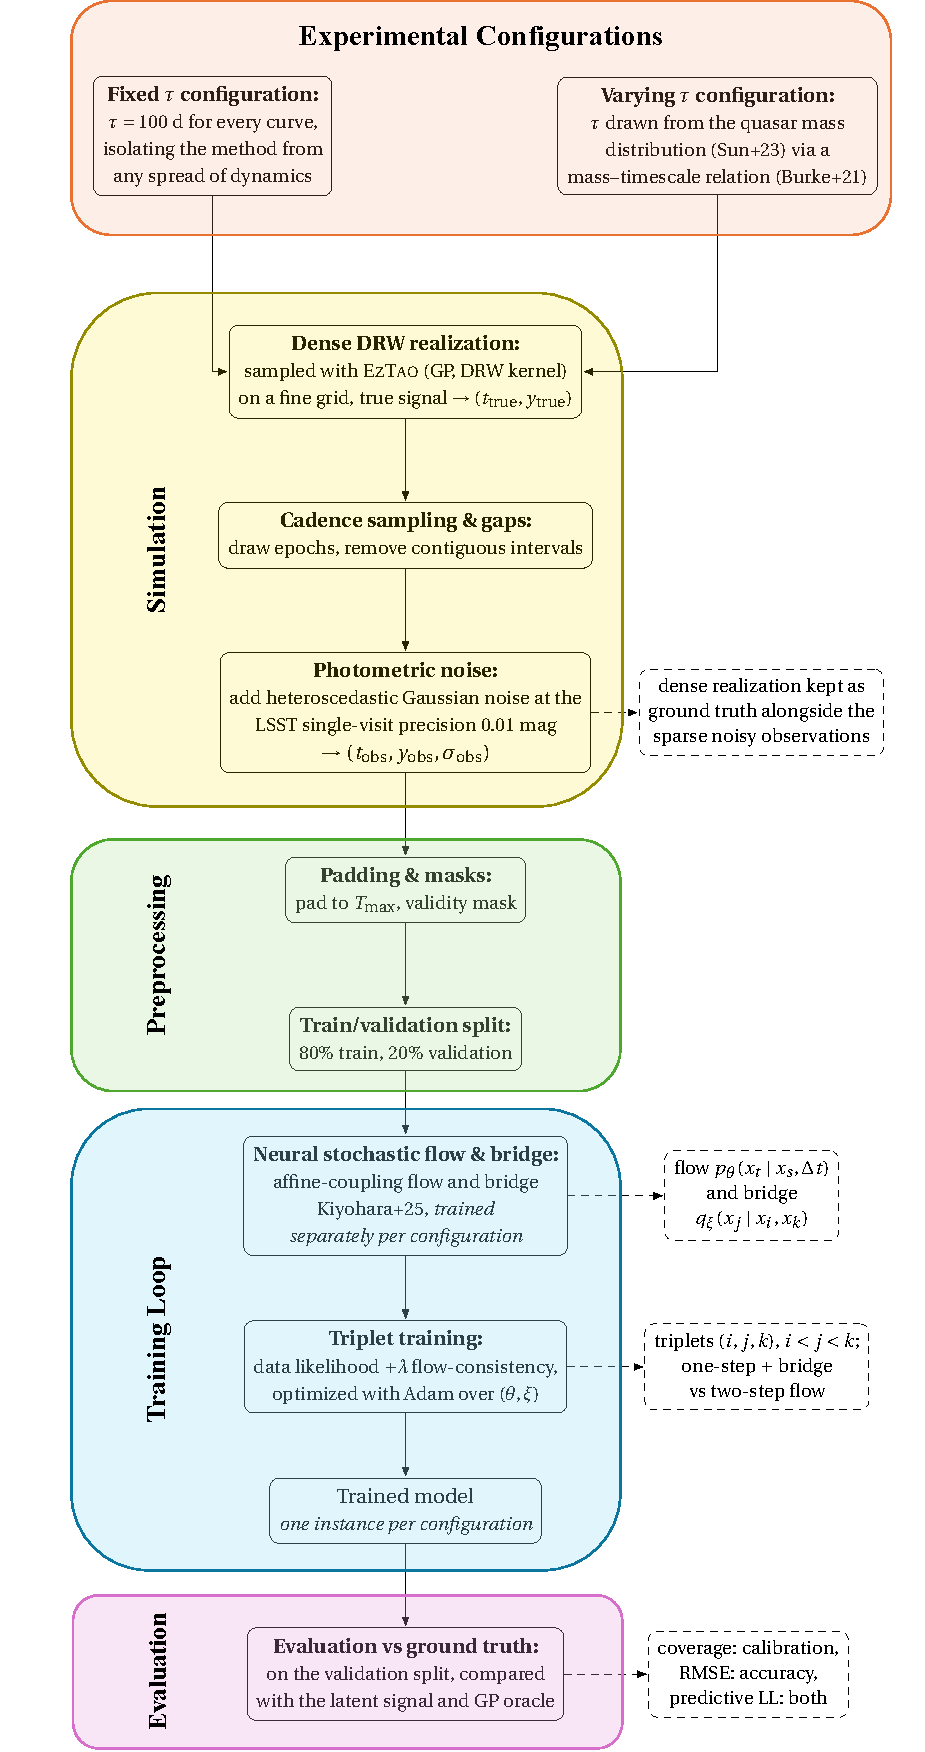
\includegraphics[height=1\textheight]{assets/5_figures/LC_FD.pdf}
    \caption[Pipeline of the idealized simulation experiments]{\label{fig:pipeline_sim} Pipeline of the idealized simulation experiments.}
\end{figure}

\section{Low Noise Simulations}
\label{sec:lownoise}

On the simulated data the reconstruction is measured against a Gaussian process with the damped random walk kernel, given the true parameters of each curve. As shown in Section \ref{ssec:transition}, conditioning the damped random walk on the observations yields a Gaussian predictive distribution in closed form. Supplied with the true timescale and amplitude, this is the Bayes-optimal predictor, since no method conditioned on the same observations can achieve a lower expected error, and it therefore sets the ceiling against which the reconstruction is measured.

\subsection{Fixed Timescale}
\label{ssec:fixedtau}

The most controlled experiment fixes the damping timescale at $\tau = 100$ d for every light curve, removing any variation in dynamics so that the behaviour of the method can be studied in isolation. The training objective converges within a few hundred steps (Figure \ref{fig:fixed_training}a).

The first quantity examined is the learned transition itself, independently of any reconstruction. The trained flow defines a transition density $p_\theta(x_{t+\Delta t} \mid x_t, \Delta t)$, and because the true transition of the damped random walk is known in closed form, the two can be compared directly. The comparison is constructed as follows. A single starting state $x_s$ is fixed, and a set of elapsed times $\Delta t$ is chosen spanning from a small fraction of the damping timescale to several times it. For each elapsed time, a large sample, here four thousand draws, is taken from the flow conditioned on $x_s$ and that elapsed time, and the empirical mean and standard deviation of the samples are formed. 

\begin{figure}[H]
    \centering
    \begin{subfigure}{\textwidth}
        \centering
        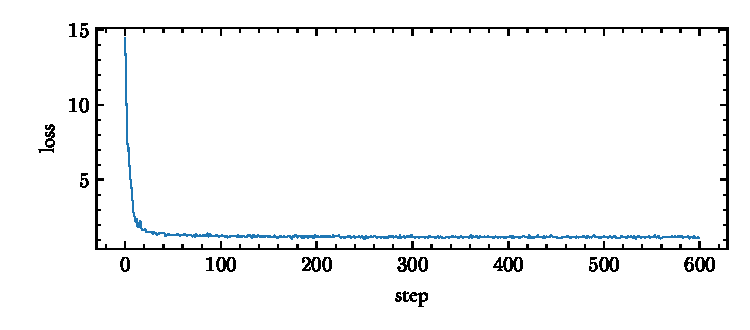
\includegraphics[width=0.7\textwidth]{assets/5_figures/FixedTauExp/Loss.pdf}
        \caption{Training loss as a function of optimization step.}
        \label{fig:loss}
    \end{subfigure}
    %\vspace{\baselineskip}
    \begin{subfigure}{0.9\textwidth}
        \centering
        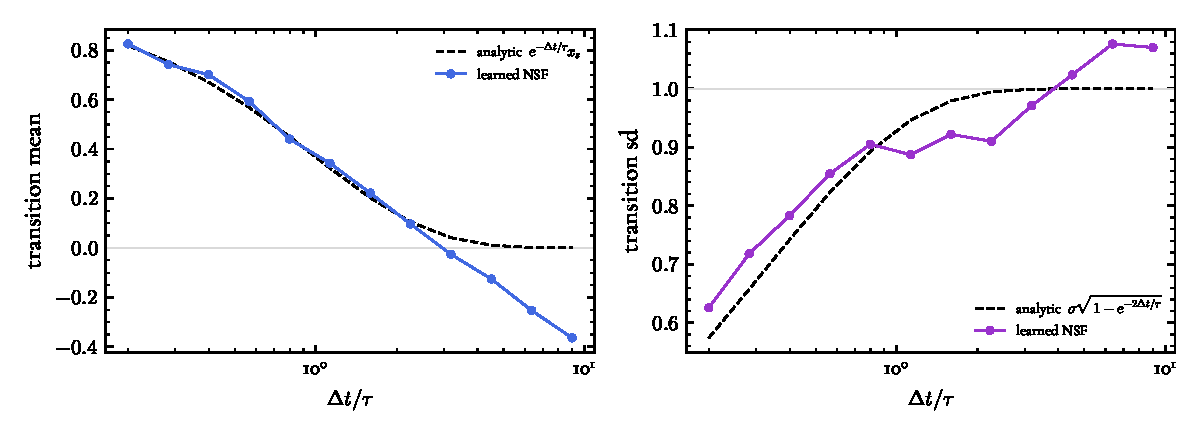
\includegraphics[width=\textwidth]{assets/5_figures/FixedTauExp/LearnedTrans.pdf}
        \caption{Mean (left) and standard deviation (right) of the learned transition, in units of the damping timescale, against the analytic damped random walk (dashed).}
        \label{fig:trans_fixed}
    \end{subfigure}
    \caption[Training and learned transition at fixed timescale]{\label{fig:fixed_training} Training and validation of the fixed-timescale model.}
\end{figure}

These are compared with the analytic mean $e^{-\Delta t/\tau}x_s$ and standard deviation $\sqrt{\sigma^2(1 - e^{-2\Delta t/\tau})}$ of Equation \ref{eq:drw_transition}, evaluated at the same elapsed times. Repeating this over the range of $\Delta t$ traces out the learned mean and standard deviation as functions of the elapsed time, which is expressed in units of the damping timescale since it is this ratio that governs the transition. The procedure is carried out by \texttt{checkTransition} (in \texttt{NSF.py}), and all quantities are computed in the normalized units in which the model is trained. Figure \ref{fig:fixed_training}b shows the result. The learned mean relaxes towards zero and the learned standard deviation grows towards its stationary value, both following the analytic curves across the whole range, so the flow has recovered the transition law of the process it was trained on. %This is a stronger check than reconstruction accuracy alone: it confirms that the model has learned the correct one-step dynamics, and not merely that it interpolates the observations well.


Applied to full light curves, the method reconstructs the signal on the dense grid between the observations, drawing two hundred samples from the bridge at twelve grid points between each consecutive pair, and returning a posterior median and a predictive interval at every point. An example is shown in Figure \ref{fig:filled_fixed}. The reconstruction follows the underlying signal through the gaps, and the interval widens across the wider gaps as the bracketing observations become less informative. The accuracy of the reconstruction is quantified by the error against the true dense realization as a function of gap width, in units of the damping timescale (Figure \ref{fig:error_fixed}). The error grows smoothly with the gap, and tracks that of the Gaussian process across the whole range, converging with it at the widest gaps, where the observations no longer constrain the signal and the correct prediction for both methods is the stationary prior. The difficulty of the reconstruction is therefore set by the size of the gap relative to the correlation length, as expected when the underlying process is recovered correctly.

\begin{figure}[H]
    \centering
    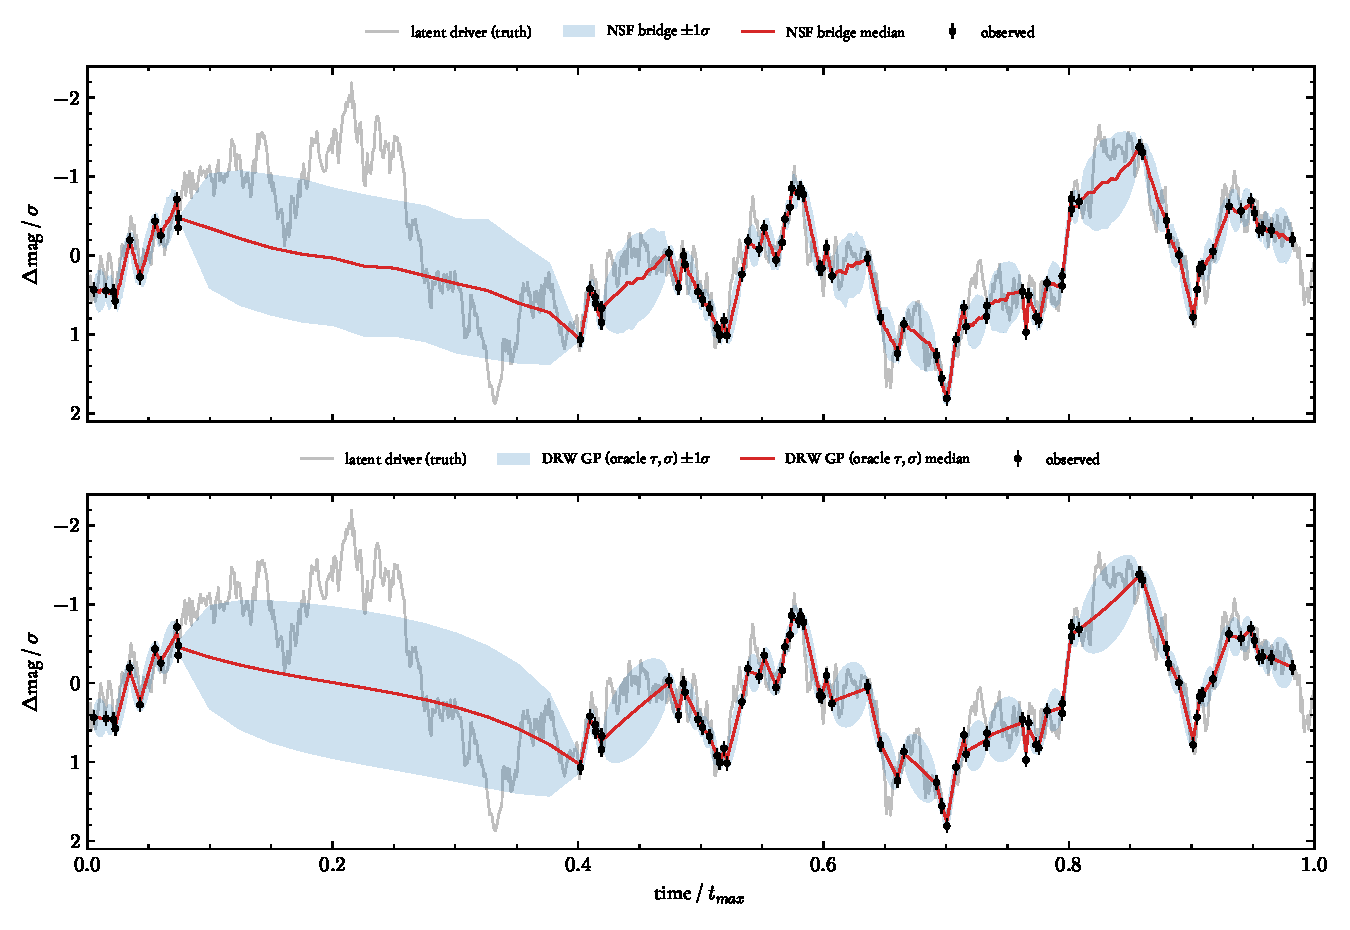
\includegraphics[width=\textwidth]{assets/5_figures/FixedTauExp/FilledLightCurve.pdf}
    \caption[Reconstruction of a fixed-timescale light curve]{\label{fig:filled_fixed} Reconstruction of a light curve from the fixed-timescale experiment, showing the posterior median (blue) and the central $68\%$ interval (shaded) against the true dense realization (grey). The observations are shown in black, and the interval widens across the gaps between them.}
\end{figure}

This is the setting in which the reconstruction and the Gaussian process agree most closely across the experiments, as expected in the absence of any spread of timescales or survey-level noise, and it serves as the reference against which the effect of each added element of realism is measured in the sections that follow.

\begin{figure}[H]
    \centering
    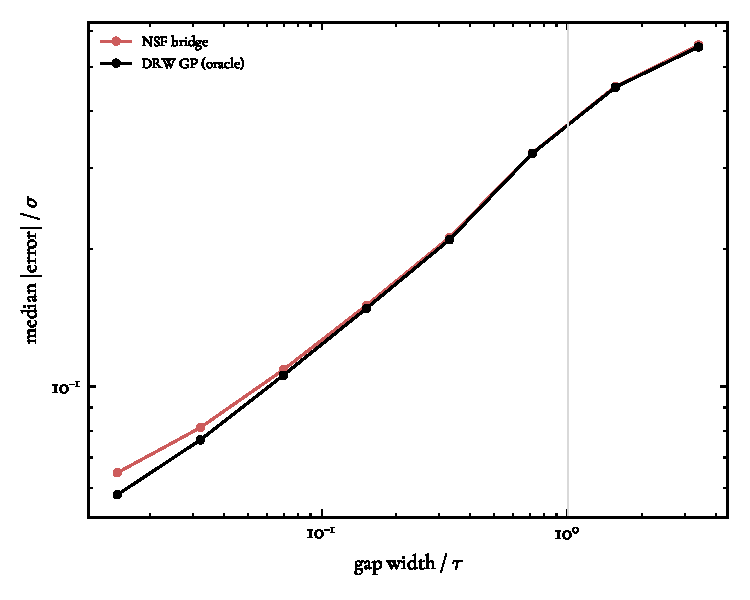
\includegraphics[width=0.6\textwidth]{assets/5_figures/FixedTauExp/Error.pdf}
    \caption[Reconstruction error against gap width at fixed timescale]{\label{fig:error_fixed} Reconstruction error as a function of gap width in units of the damping timescale, compared with the Gaussian process. The two track each other and converge at the widest gaps, where the correct prediction is the prior.}
\end{figure}

\pagebreak

\subsection{Varying Timescale}
\label{ssec:varytau}

The timescale is next drawn from the physically motivated distribution of Section \ref{sec:tausampling}, so that each light curve carries its own damping timescale and the flow is trained on a mixture of dynamics rather than a single one. This is the more demanding and more realistic test, since the model must now represent a family of transitions rather than a single one, with the timescale of each curve inferred implicitly from its observations.

Because the transition now depends on the timescale of the individual curve, there is no longer a single learned transition to compare against the analytic form. It is instead evaluated at the median timescale of the distribution, using the same procedure as before with the damping timescale set to the median value. The learned transition remains close to the analytic one over most of the range, departing only at the longest separations, where the mean reaches $-0.30$ at nine damping timescales rather than relaxing to zero, and the standard deviation settles near $1.11$ rather than unity (Figure \ref{fig:trans_vary}). This residual is small and appears at the separations that are least represented in the training data, since gaps spanning many damping timescales are rare even when the span of the sampled triplets is drawn log-uniformly. The same slight overshoot of the mean past zero and inflation of the standard deviation reappear, greatly amplified, once survey-level noise is introduced in the ZTF experiments, where they become the signature of the model's difficulty with noisy observations.

\begin{figure}[H]
    \centering
    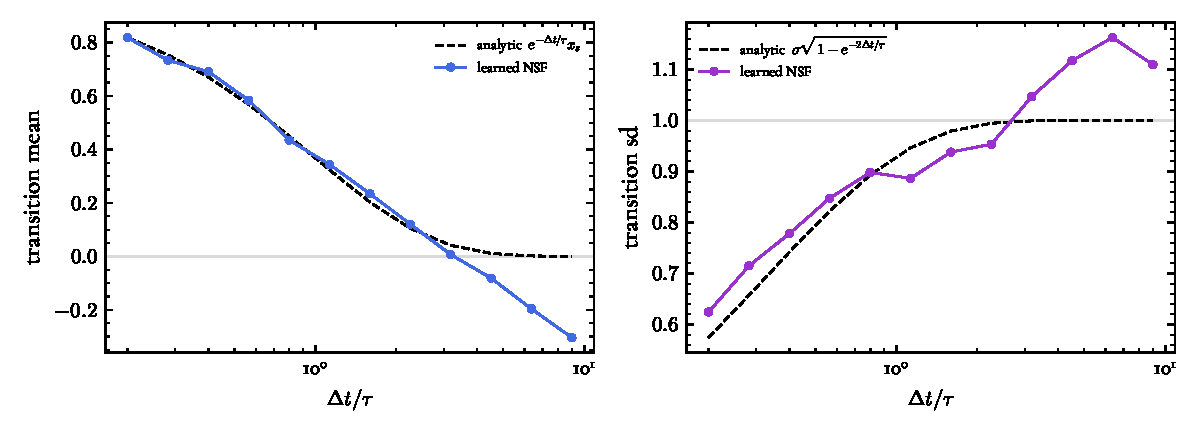
\includegraphics[width=\textwidth]{assets/5_figures/VaryTauExp/LearnedTransMedian.pdf}
    \caption[The learned transition at varying timescale]{\label{fig:trans_vary} The mean (left) and standard deviation (right) of the learned transition, evaluated at the median damping timescale, compared with the analytic damped random walk (dashed). A small residual bias remains at the longest separations.}
\end{figure}

In reconstruction the method stays close to the Bayes-optimal reference across the whole distribution of timescales. Each validation curve is reconstructed in the same way and scored on its gap interiors against its own true signal, with the Gaussian process baseline given that curve's true parameters, and the results are aggregated over the validation set. The method reaches a median coverage of $0.61$ at the $68\%$ level, with a central range of $[0.55, 0.67]$ across curves, against $0.70\ [0.66, 0.73]$ for the Gaussian process, and a median RMSE of $0.172\ [0.151, 0.204]$ against $0.167\ [0.144, 0.200]$, placing the reconstruction about $3\%$ above the optimal reference in error. The coverage varies systematically with the timescale of the curve. Splitting the validation set at the median timescale, the curves with shorter timescales reach a median coverage of $0.57$ and those with longer timescales $0.64$. This follows from the sampling. A short timescale decorrelates faster, so for a fixed cadence the gaps span more correlation lengths and the reconstruction is harder, whereas a long timescale keeps neighbouring epochs correlated and the reconstruction is better constrained.

Figure \ref{fig:filled_vary} compares the reconstruction with the Gaussian process on the same light curve. The two are closely matched where the observations are dense, and across the wider gaps both widen into broad intervals that follow the same shape, with the reconstruction and the oracle assigning almost the same uncertainty to the unobserved stretches. The individual Monte Carlo samples that make up such a reconstruction were shown earlier in Figure \ref{fig:mcsamples}.

\begin{figure}[H]
    \centering
    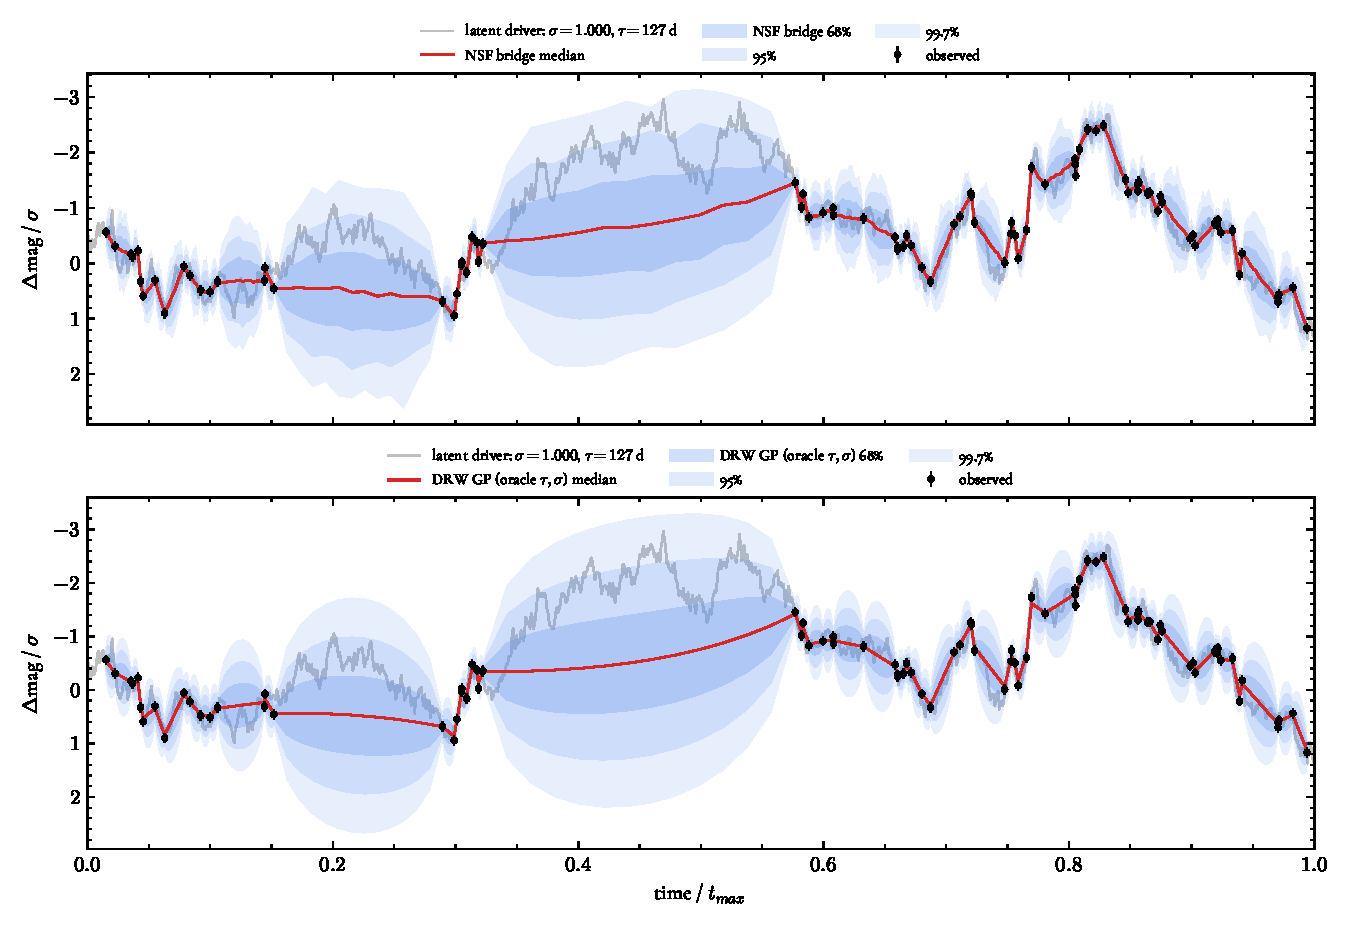
\includegraphics[width=\textwidth]{assets/5_figures/VaryTauExp/FilledLightCurve.pdf}
    \caption[Reconstruction of a varying-timescale light curve]{\label{fig:filled_vary} Reconstruction of a varying-timescale validation curve by the neural stochastic flow (top) and the Gaussian process given the true parameters (bottom), shown against the true dense realization (grey), with the observations in black. Each shows the posterior median (red) and the nested central $68$, $95$, and $99.7\%$ intervals (shaded). The two assign closely matching uncertainty across the gaps.}
\end{figure}

%%%%%%%%%%%
\clearpage

\begin{figure}[p]
    \centering
    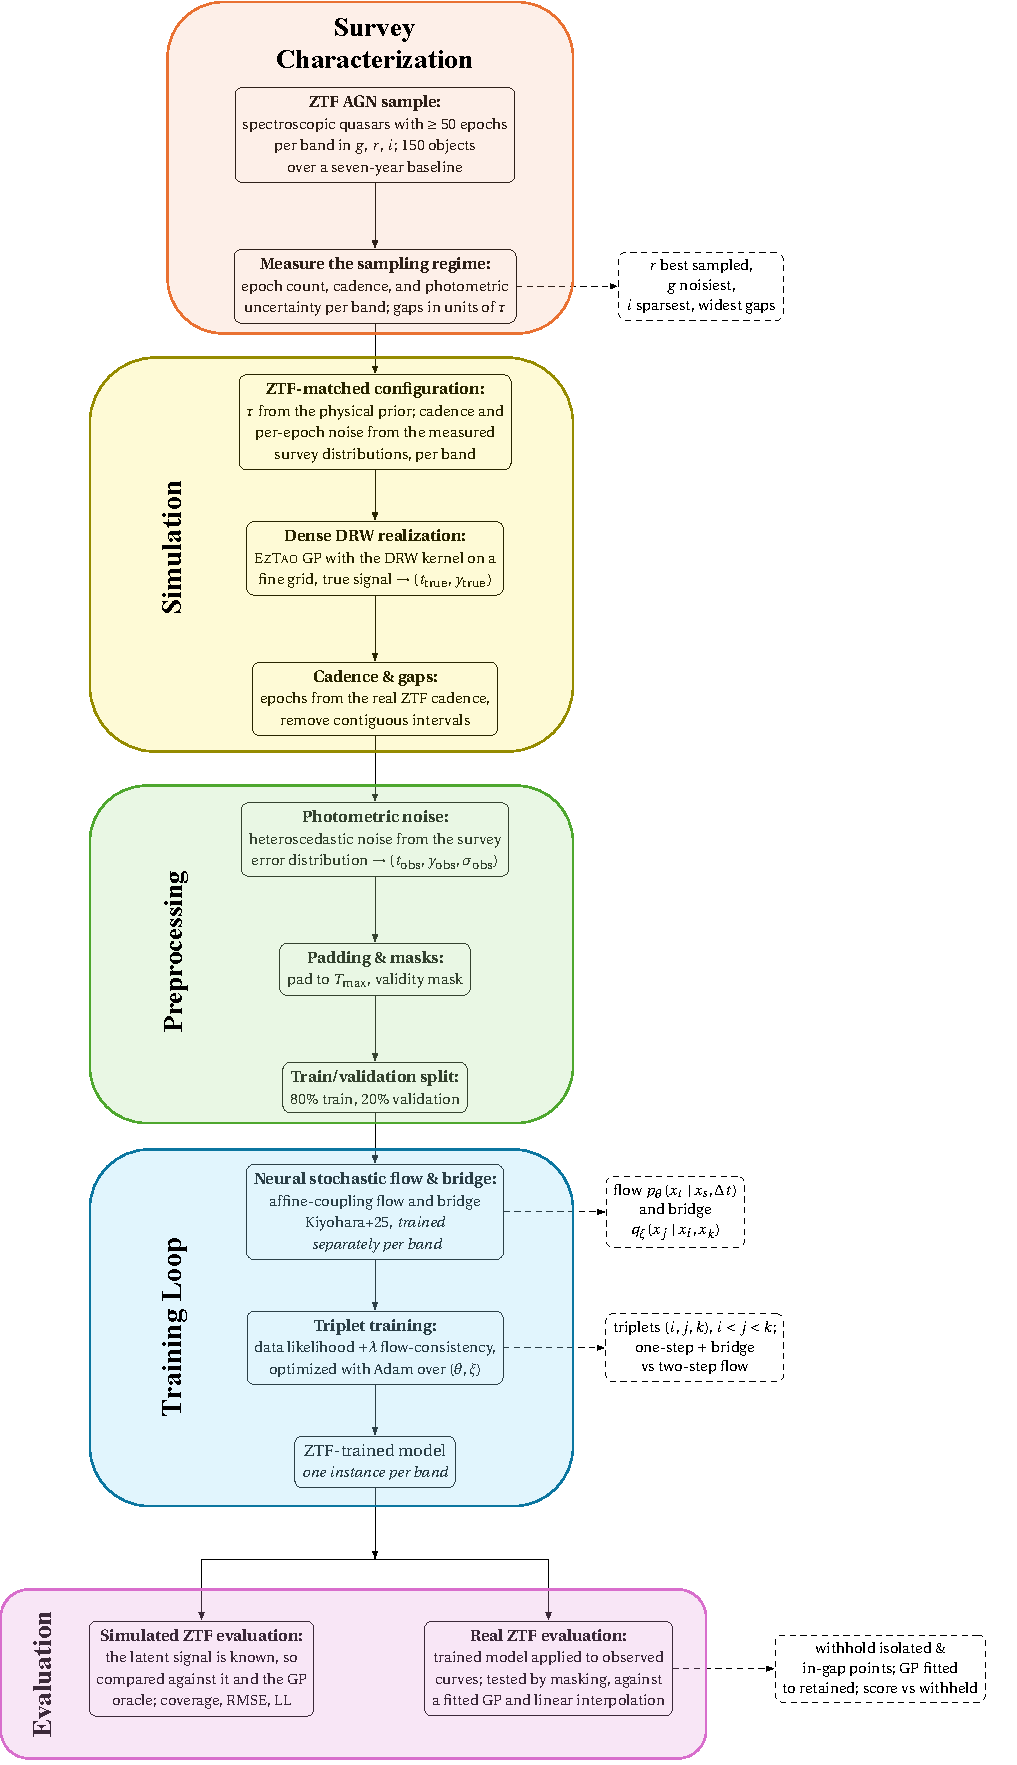
\includegraphics[height=1\textheight]{assets/5_figures/ZTF_FD.pdf}
    \caption[Pipeline of the ZTF experiments]{\label{fig:pipeline_ztf} Pipeline of the ZTF experiments.}
\end{figure}
\clearpage


\section{ZTF Experiments}
\label{sec:ztf}

% add the specific scripts used and differences between this and the previous

The sampling regime that the simulations must reproduce is measured from a sample of real AGN. Starting from a catalogue of spectroscopically confirmed quasars, light curves are drawn from ZTF in the $g$, $r$, and $i$ bands. Within each band, observations separated by less than $0.3$ days are treated as duplicates and only the first is kept, since on the timescales of interest such closely spaced points are almost perfectly correlated under the damped random walk and add little information while distorting the cadence statistics. Objects are retained only if at least $50$ epochs remain in each band, giving a sample of $150$ AGN over a baseline of roughly seven years. An example is shown in Figure \ref{fig:ztfexample}, with the irregular cadence and seasonal gaps characteristic of a ground-based survey.

\begin{figure}[H]
    \centering
    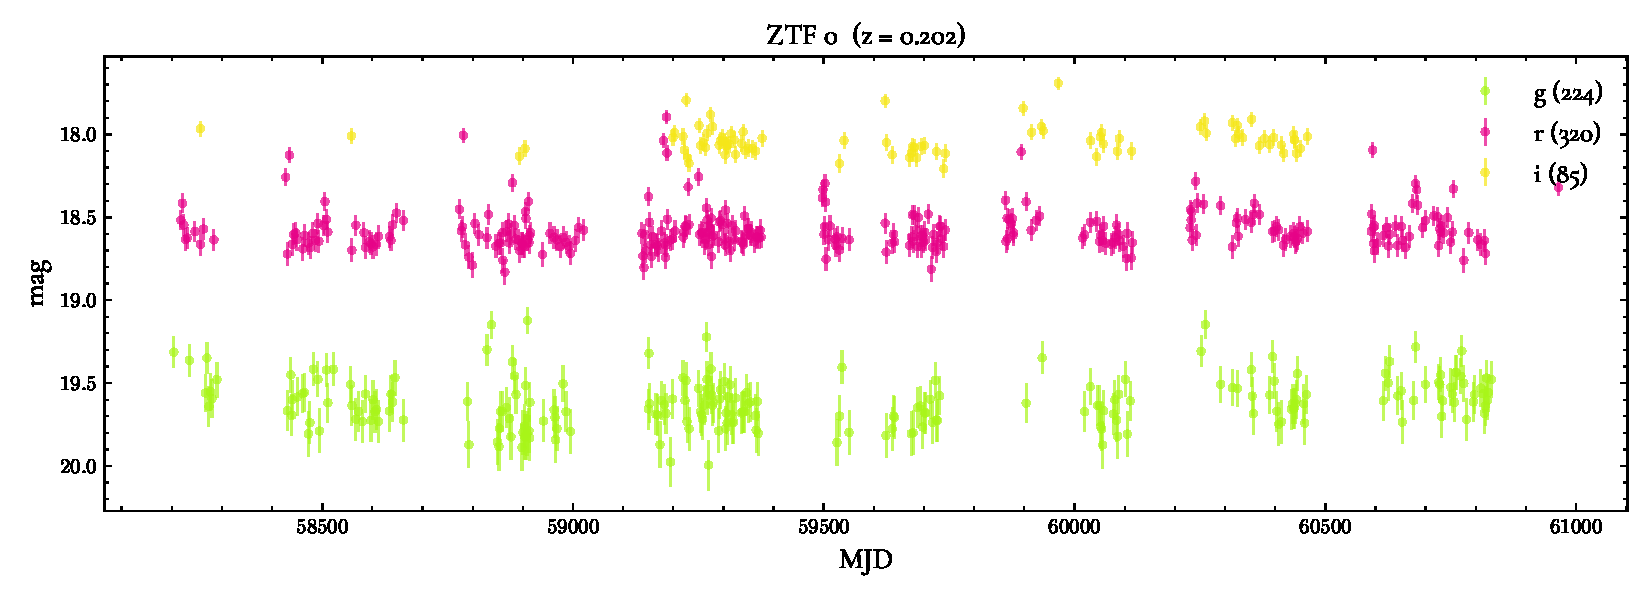
\includegraphics[width=0.9\textwidth]{assets/5_figures/ZTF/ZTF_real_lc_example.pdf}
    \caption[An example real ZTF light curve]{\label{fig:ztfexample} A real ZTF light curve of one AGN in the sample, showing the irregular cadence and seasonal gaps of a ground-based survey.}
\end{figure}

The distributions of the number of epochs, the cadence, and the photometric uncertainty differ between the three bands (Figure \ref{fig:ztfstats}). The $r$ band is the most densely sampled, the $g$ band carries the largest photometric uncertainties, since ZTF is shallower in $g$, and the $i$ band is the most sparsely sampled. These per-band distributions are used directly to construct the ZTF-matched simulations, so that each simulated band inherits the cadence and noise of its real counterpart.

\begin{figure}[H]
    \centering
    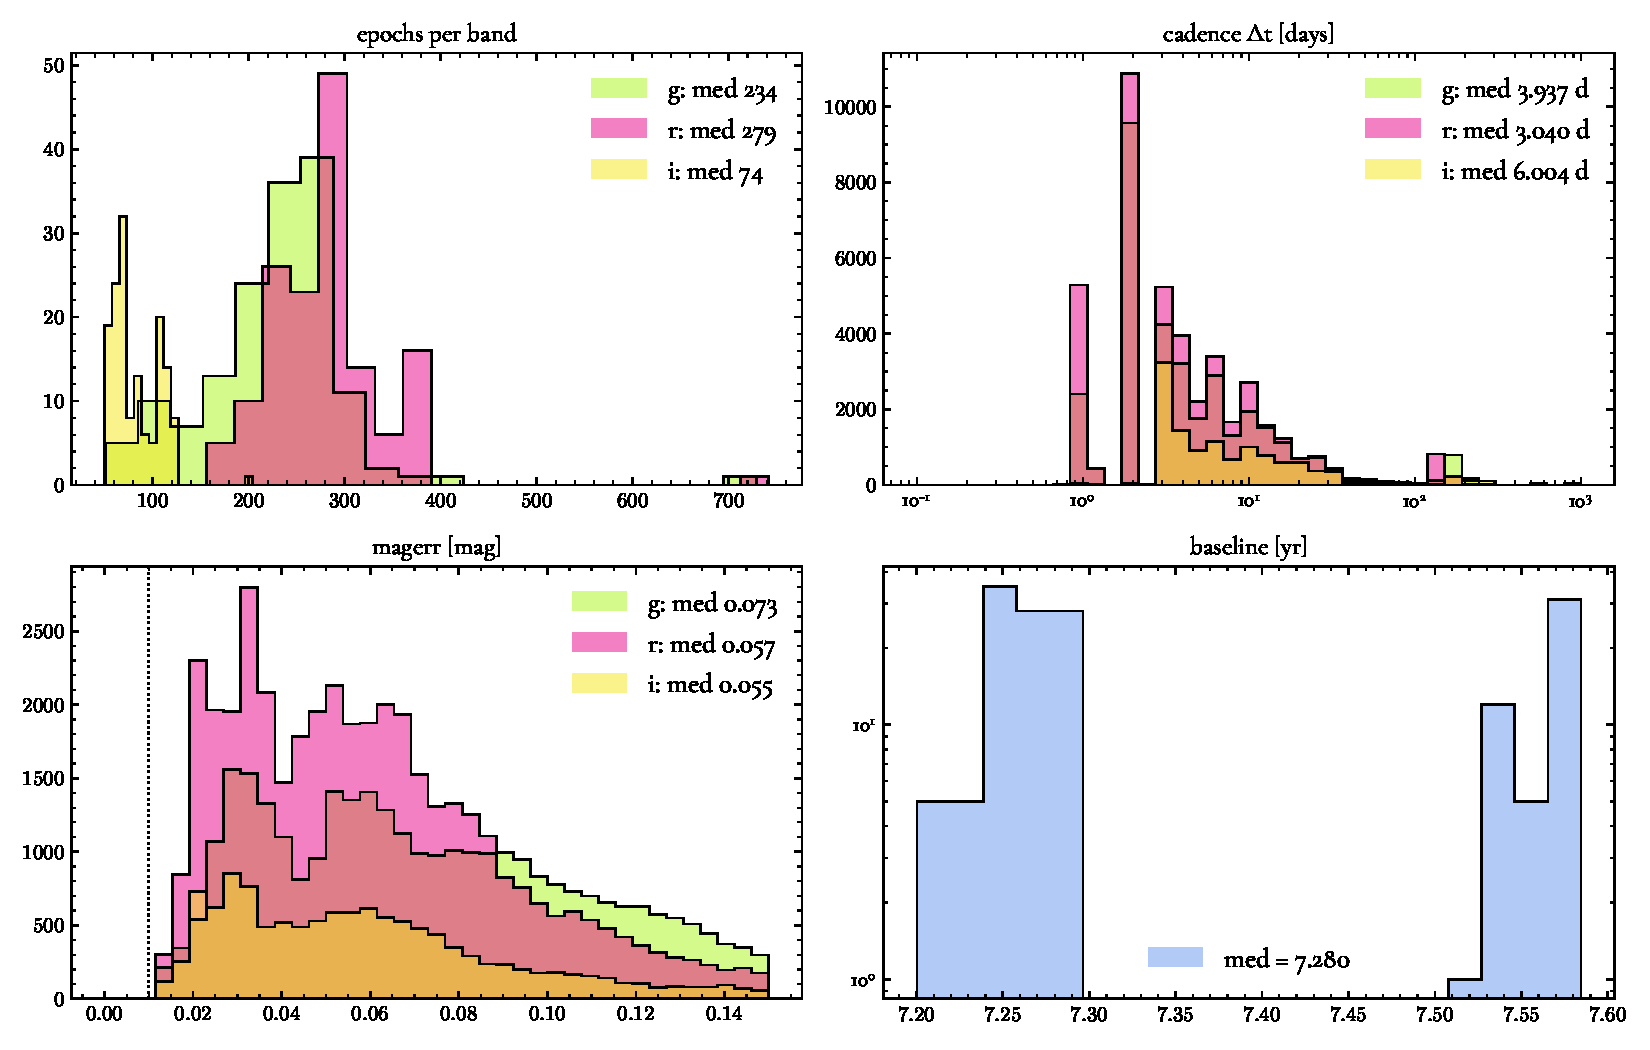
\includegraphics[width=0.7\textwidth]{assets/5_figures/ZTF/ZTF_statistics.pdf}
    \caption[Sampling and noise statistics of the ZTF sample]{\label{fig:ztfstats} Distributions of the number of epochs, cadence, and photometric uncertainty across the $150$ ZTF AGN in the $g$, $r$, and $i$ bands.}
\end{figure}

The quantity that controls the difficulty of reconstruction is the size of the gaps relative to the damping timescale, since a damped random walk loses memory as $e^{-\Delta t/\tau}$ and it is gaps comparable to or larger than $\tau$ that make reconstruction non-trivial. Expressed in these units the three bands probe noticeably different regimes (Figure \ref{fig:ztfregime}). In the $g$ band the median largest gap per curve is $1.24\,\tau$, with $73\%$ of curves containing a gap wider than the damping timescale; in the $r$ band the median largest gap is $1.05\,\tau$, with $56\%$ exceeding $\tau$; and in the $i$ band the median largest gap is $2.10\,\tau$, with $89\%$ exceeding $\tau$ and a tail reaching almost seven damping timescales. The $i$ band therefore contains the widest gaps, some large enough that the endpoints retain essentially no information about the intervening signal, and it is the band in which single-band reconstruction is most strongly limited.

An example of a simulated light curve from the ZTF-matched configuration is shown in Figure \ref{fig:ztfsim_example}, reproducing the cadence and noise of the corresponding real band.
 
\section{Calibration on Simulated ZTF Data}
\label{sec:ztfnoise}

Trained and evaluated on light curves matched to the ZTF regime, the method continues to reconstruct the underlying signal but its predictive intervals become badly overconfident. To establish that this is a property of the model rather than of a particular training run, the training is repeated across five random seeds; the results are shown in Table \ref{tab:seeds}. The coverage at the $68\%$ level is far below nominal in every band, at $0.30$, $0.33$, and $0.42$ in $g$, $r$, and $i$, and the scatter across seeds is small, so the overconfidence is systematic. The predictive log-likelihood worsens sharply with the noise level of the band, from $-3.29$ in the least noisy band to $-10.63$ in the noisiest, since the noisiest band produces the narrowest intervals relative to the scatter of the truth and is penalized most heavily for the points that fall outside them.

\begin{figure}[H]
    \centering
    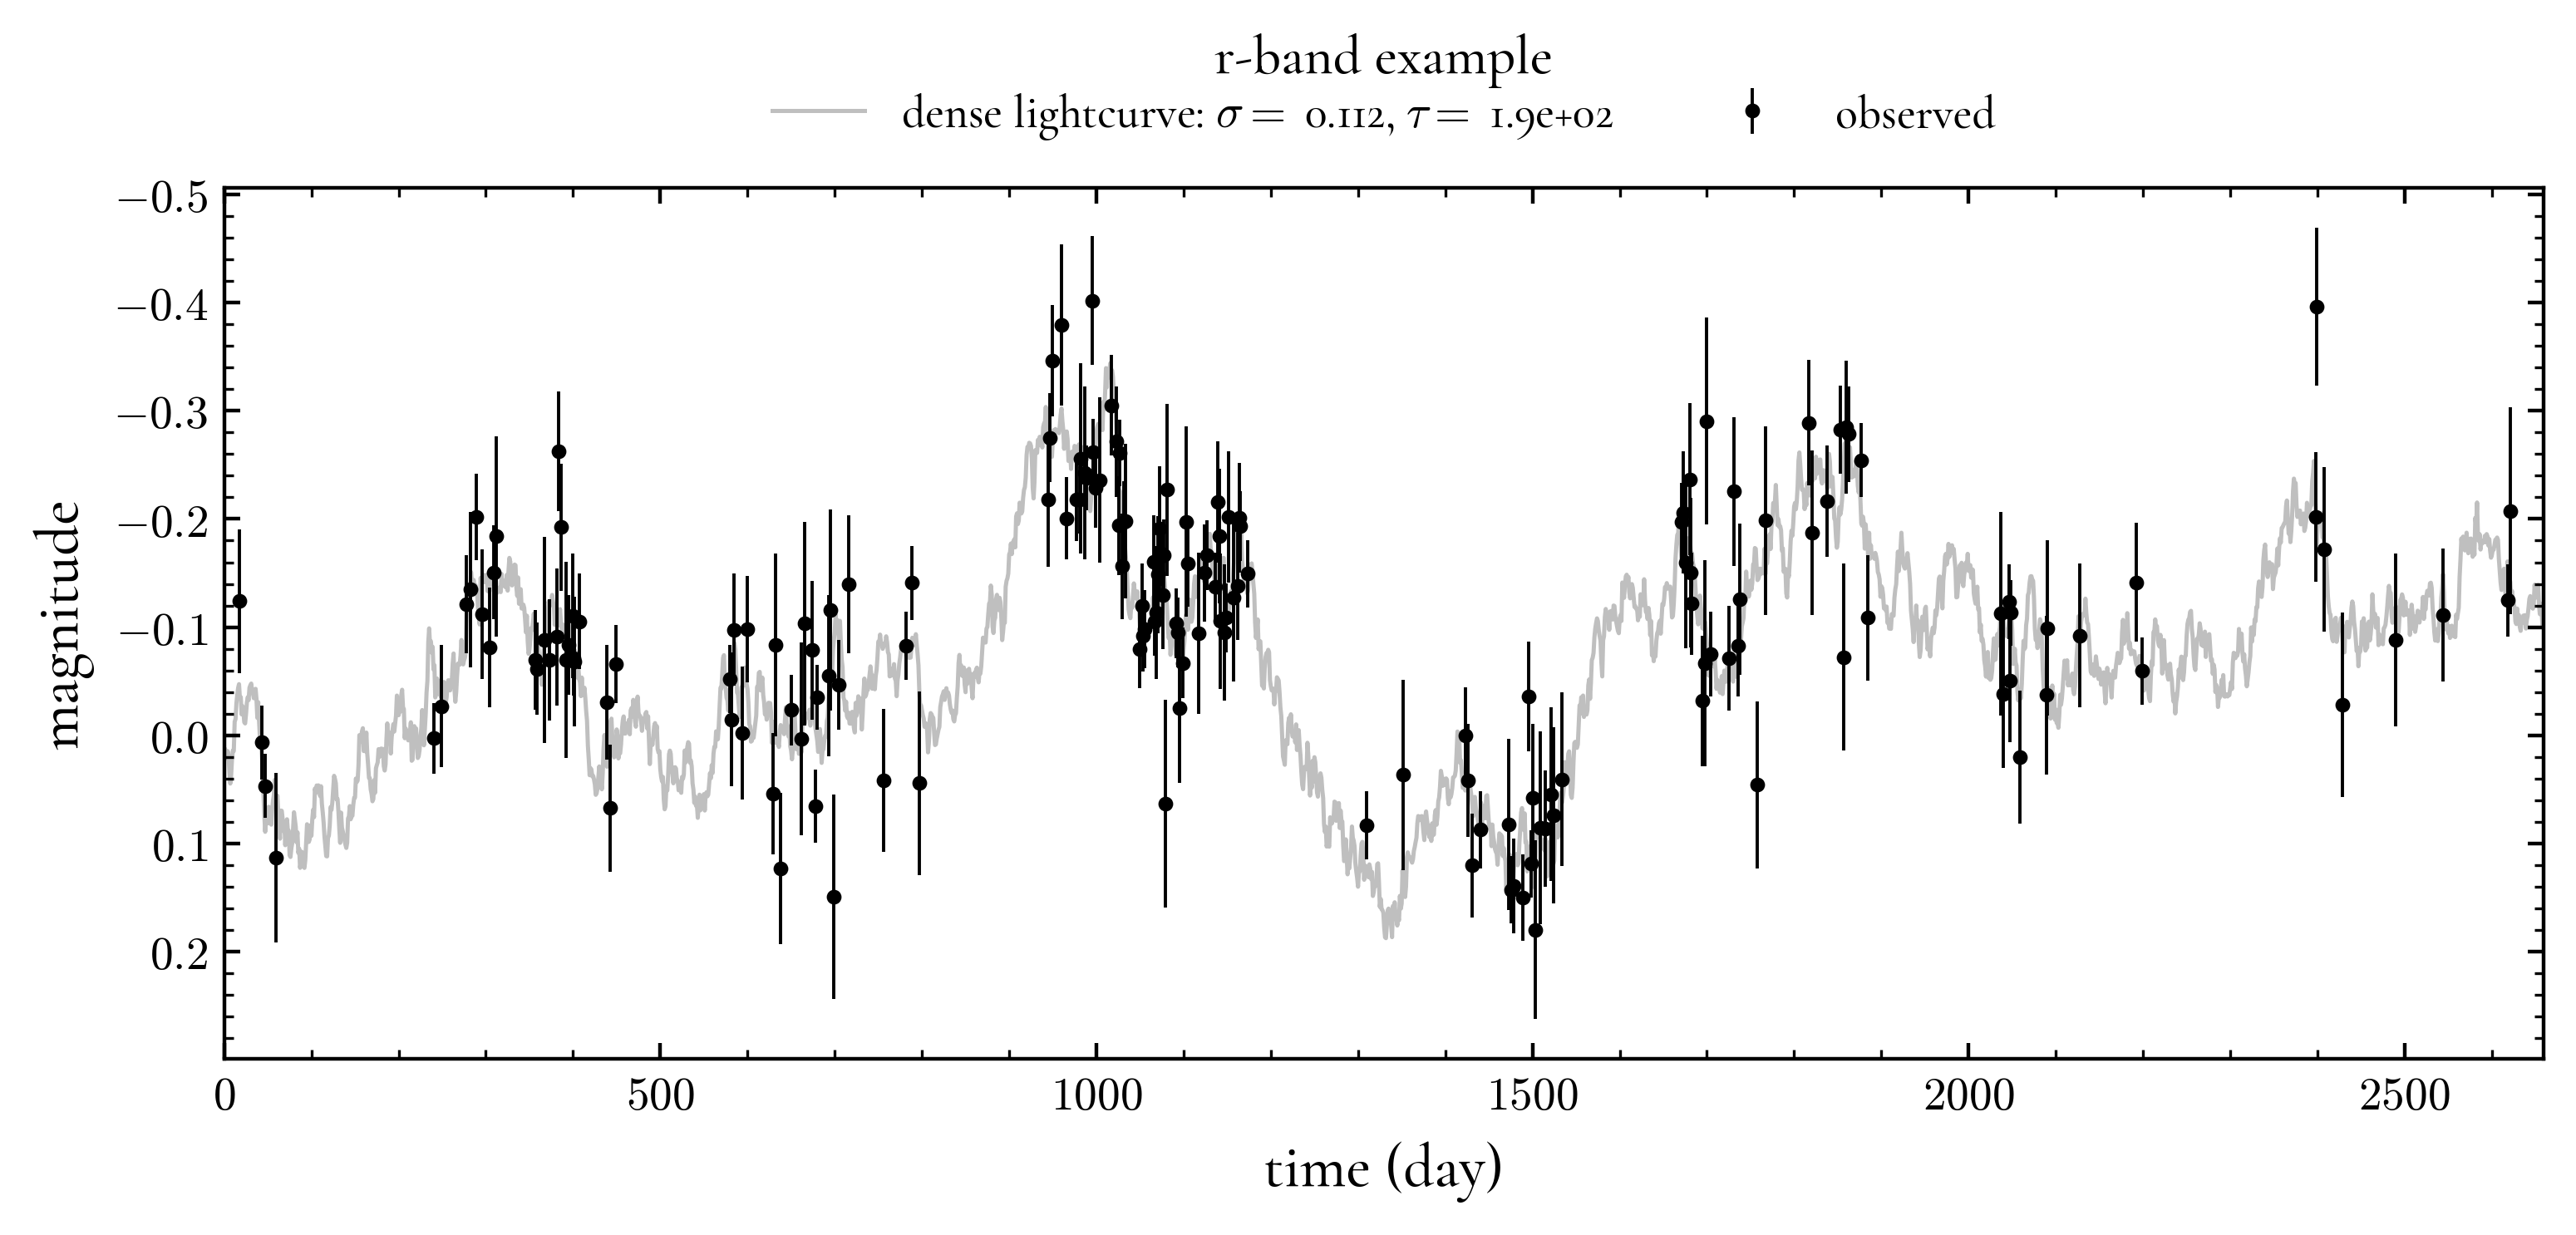
\includegraphics[width=\textwidth]{assets/5_figures/ZTF/ZTF_simulated_lc_r.png}
    \caption[An example simulated ZTF-matched light curve]{\label{fig:ztfsim_example} A simulated light curve from the ZTF-matched configuration, with the dense underlying realization and the sparse noisy observations drawn from it at the survey cadence.}
\end{figure}


\begin{figure}[H]
    \centering
    \begin{subfigure}{\textwidth}
        \centering
        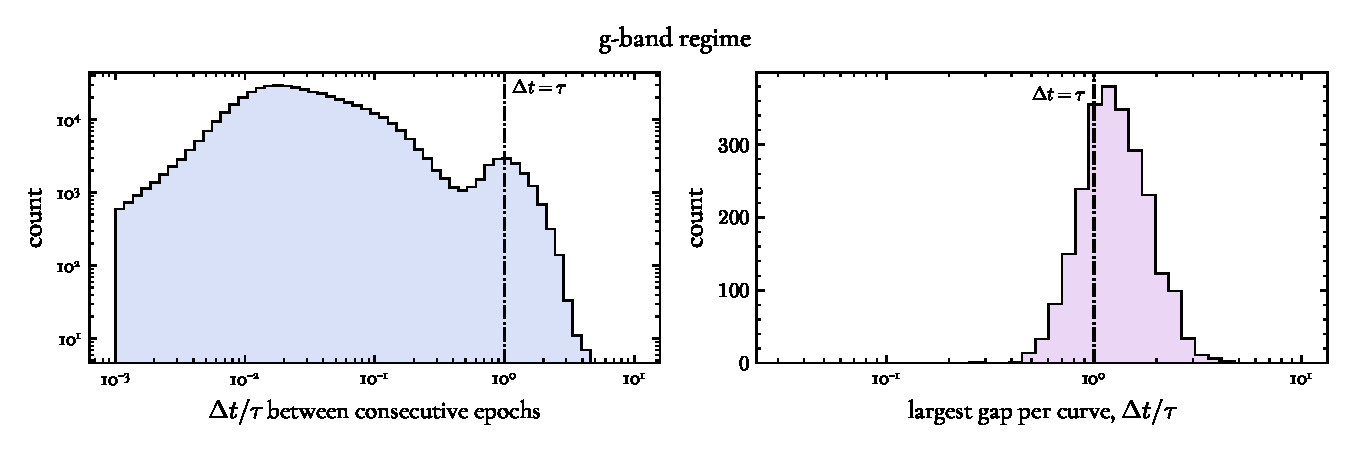
\includegraphics[width=0.82\textwidth]{assets/5_figures/ZTF/simulation_g_regime.pdf}
        \caption{$g$ band}
    \end{subfigure}
    \begin{subfigure}{\textwidth}
        \centering
        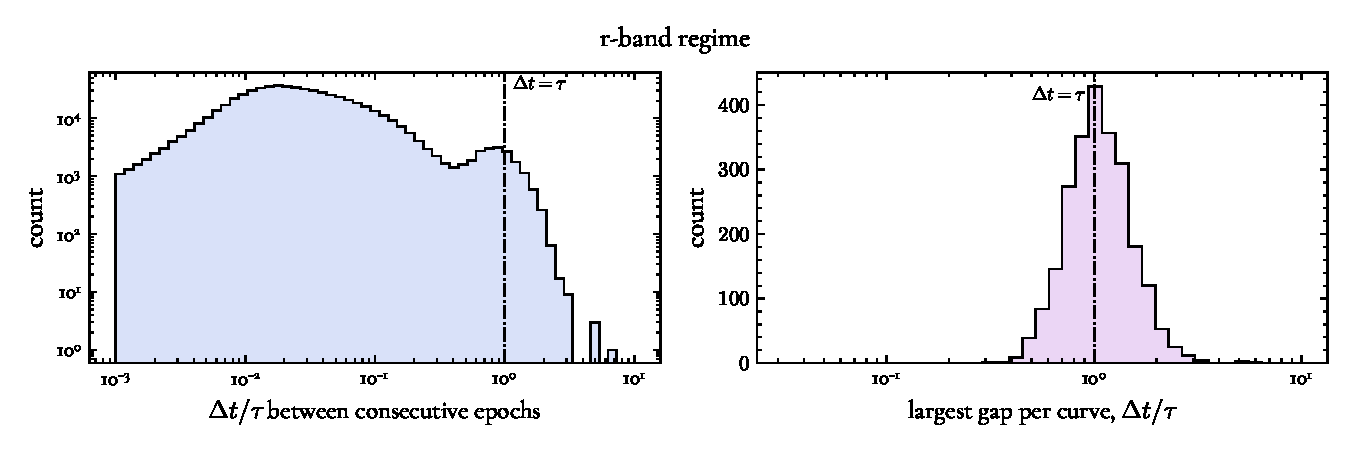
\includegraphics[width=0.82\textwidth]{assets/5_figures/ZTF/simulation_r_regime.pdf}
        \caption{$r$ band}
    \end{subfigure}
    \begin{subfigure}{\textwidth}
        \centering
        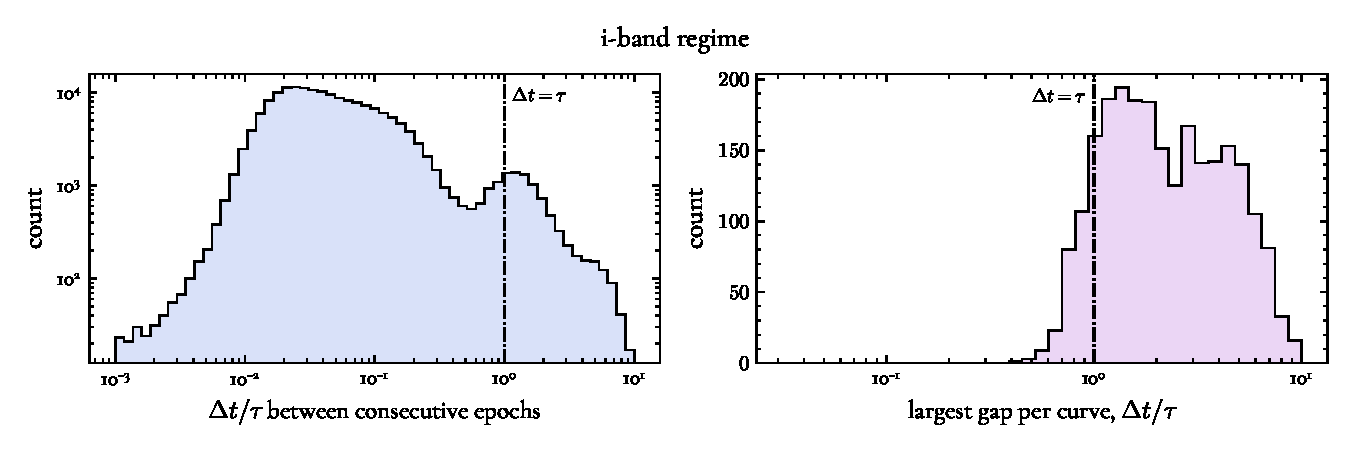
\includegraphics[width=0.82\textwidth]{assets/5_figures/ZTF/simulation_i_regime.pdf}
        \caption{$i$ band}
    \end{subfigure}
    \caption[Sampling regime of the ZTF-matched light curves per band]{\label{fig:ztfregime} The spacing between consecutive epochs (left) and the single largest gap per curve (right), in units of the damping timescale, for the ZTF-matched simulations in each band. The line marks $\Delta t = \tau$.}
\end{figure}

\begin{table}[H]
\centering
\caption[Reconstruction performance across seeds on ZTF-matched data]{\label{tab:seeds} Median coverage at the $68\%$ level, RMSE, and predictive log-likelihood on the ZTF-matched validation set, as mean and standard deviation across five training seeds.}
\begin{tabular}{lccc}
\hline
\noalign{\smallskip}
Band & Coverage @ $68\%$ & RMSE & Predictive LL \\
\noalign{\smallskip}
\hline
\noalign{\smallskip}
$g$ & $0.301 \pm 0.026$ & $0.569 \pm 0.004$ & $-10.63 \pm 2.34$ \\
$r$ & $0.331 \pm 0.020$ & $0.456 \pm 0.003$ & $-8.84 \pm 1.43$ \\
$i$ & $0.419 \pm 0.020$ & $0.466 \pm 0.002$ & $-3.29 \pm 0.44$ \\
\noalign{\smallskip}
\hline
\end{tabular}
\end{table}

The overconfidence is present at every level of the predictive interval. Table \ref{tab:multilevel} compares the empirical coverage of the reconstruction with that of the Gaussian process given the true parameters at four nominal levels. The Gaussian process is close to calibrated throughout, its empirical coverage matching each nominal level, while the reconstruction falls short at all of them, reaching only $0.46$ where $0.90$ is expected in the $g$ band. The RMSE is a factor of roughly two larger than that of the Gaussian process in every band, so the method loses accuracy as well as miscalibrating its uncertainty.

The origin of the overconfidence is visible in the learned transition. Figure \ref{fig:trans_ztf} repeats the transition comparison for models trained in the ZTF regime, in each band.

\begin{table}[H]
\centering
\caption[Coverage at multiple levels on ZTF-matched data]{\label{tab:multilevel} Empirical coverage at four nominal levels, with RMSE, for the reconstruction and the Gaussian process given the true parameters, on the ZTF-matched validation set.}
\begin{tabular}{llccccc}
\hline
\noalign{\smallskip}
Band & Method & \multicolumn{4}{c}{Coverage at nominal level} & RMSE \\
\noalign{\smallskip}
& & $0.50$ & $0.68$ & $0.90$ & $0.95$ & \\
\noalign{\smallskip}
\hline
\noalign{\smallskip}
\multirow{2}{*}{$g$} & NSF & $0.21$ & $0.31$ & $0.46$ & $0.51$ & $0.572$ \\
                     & GP  & $0.51$ & $0.68$ & $0.89$ & $0.94$ & $0.296$ \\
\noalign{\smallskip}
\multirow{2}{*}{$r$} & NSF & $0.23$ & $0.33$ & $0.50$ & $0.56$ & $0.458$ \\
                     & GP  & $0.51$ & $0.69$ & $0.90$ & $0.94$ & $0.264$ \\
\noalign{\smallskip}
\multirow{2}{*}{$i$} & NSF & $0.31$ & $0.43$ & $0.61$ & $0.67$ & $0.470$ \\
                     & GP  & $0.50$ & $0.67$ & $0.89$ & $0.94$ & $0.318$ \\
\noalign{\smallskip}
\hline
\end{tabular}
\end{table}

The agreement with the analytic transition is now lost, the learned mean overshoots, passing below zero instead of relaxing to it, and the learned standard deviation inflates to roughly $1.33$ and fails to saturate at unity. The dynamics have not been cleanly recovered as the bridge might be anchoring too tightly to the noisy observations at the gap endpoints, treating each noisy magnitude as if it were the true signal, a reconstruction pulled towards the noise.

The reconstruction error still grows smoothly with gap width (Figure \ref{fig:error_ztf}). Second, the coverage somewhat worsens as the number of epochs per curve increases (Figure \ref{fig:calib_sampling}). More epochs would ordinarily be expected to improve a reconstruction, but here a denser light curve supplies more noisy observations for the bridge to hold on to, not more usable information. The same effect appears across the bands, the sparsely sampled $i$ band being the least overconfident. A model that weighted observations by their individual uncertainties would improve with more epochs rather than degrade, so this dependence points directly at the absence of such a mechanism.

\begin{figure}[H]
    \centering
    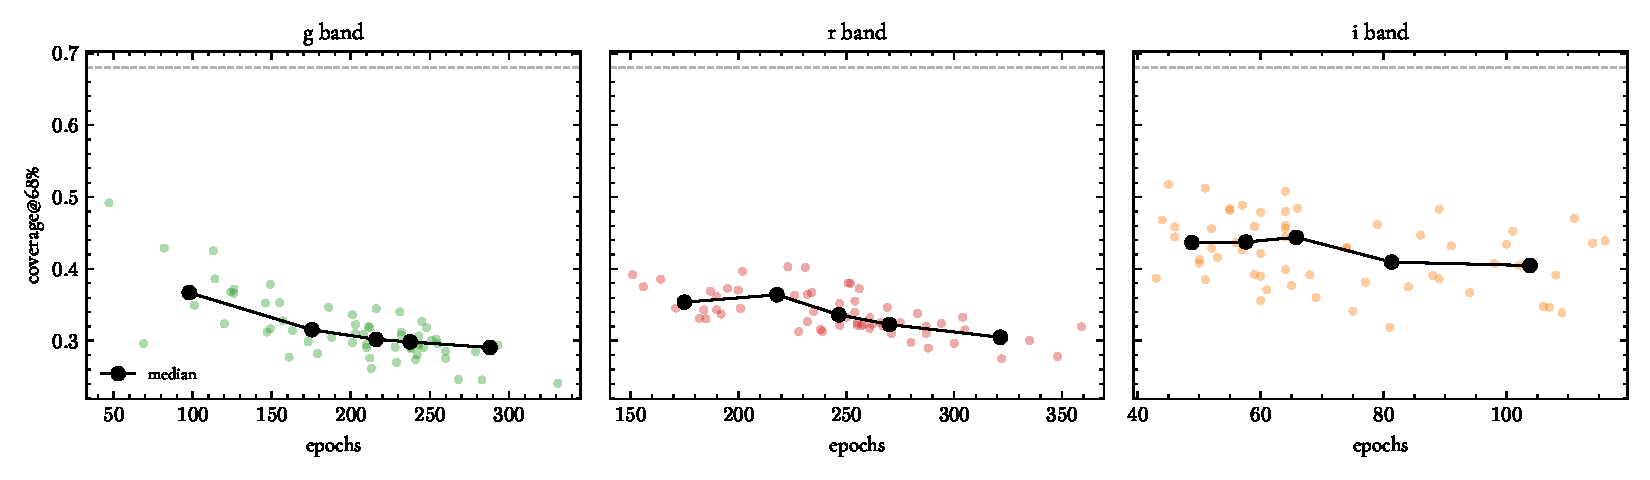
\includegraphics[width=\textwidth]{assets/5_figures/ZTF/calibrationvsSN.pdf}
    %\rule{0.85\textwidth}{0.35\textheight} % PLACEHOLDER 
    \caption[Calibration against sampling in the ZTF regime]{\label{fig:calib_sampling} Coverage as a function of the number of epochs per curve, for the three ZTF bands where coverage worsens slightly as the number of epochs grows.}
\end{figure}


\begin{figure}[H]
    \centering
    \begin{subfigure}{\textwidth}
        \centering
        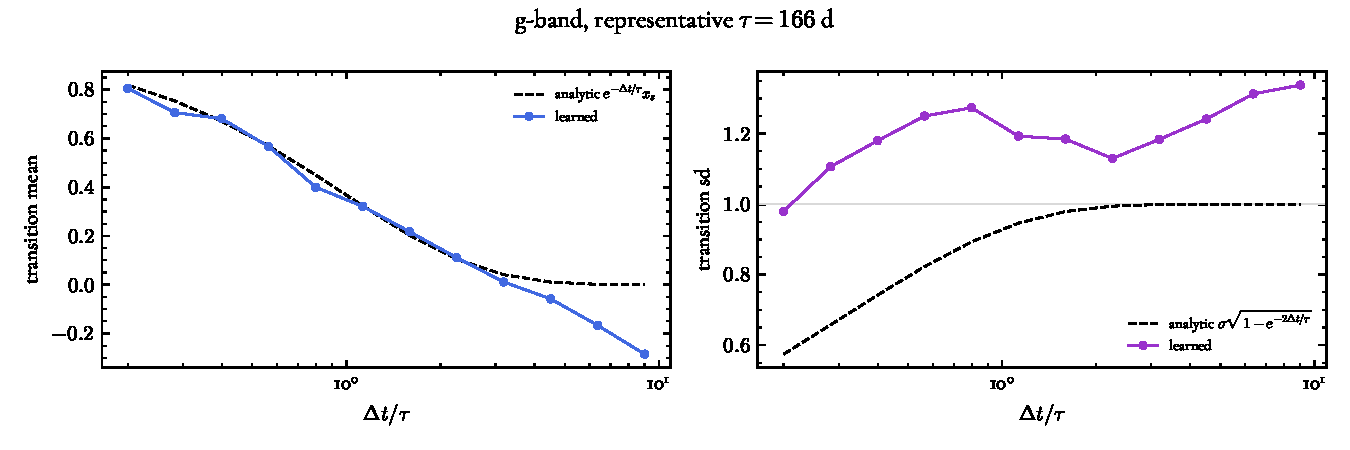
\includegraphics[width=0.9\textwidth]{assets/5_figures/ZTF/ZTF_LearnedTransg.pdf}
        \caption{$g$ band}
        \label{fig:trans_ztf_g}
    \end{subfigure}

    \begin{subfigure}{\textwidth}
        \centering
        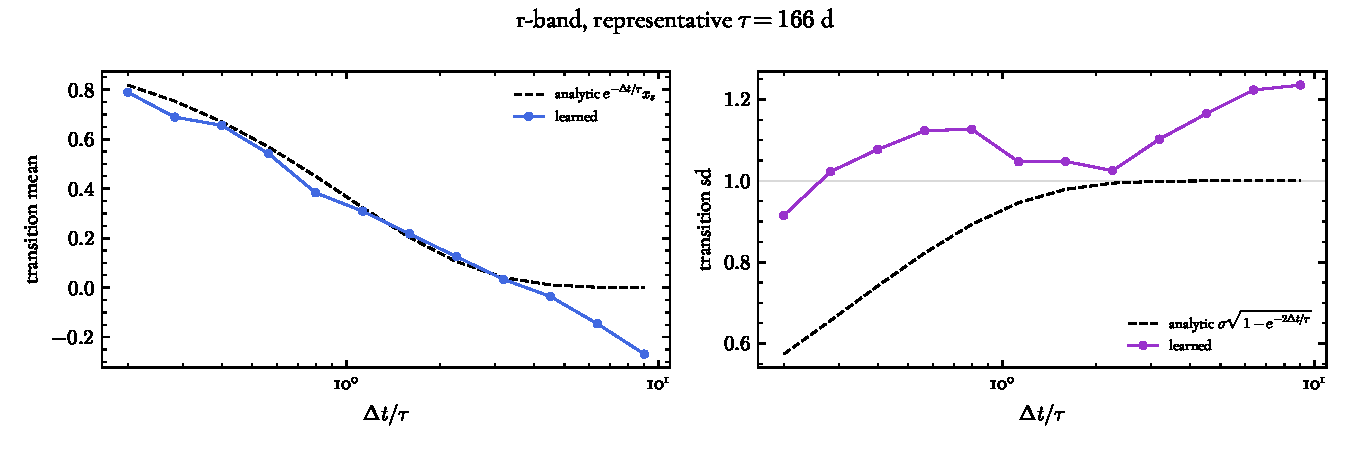
\includegraphics[width=0.9\textwidth]{assets/5_figures/ZTF/ZTF_LearnedTransr.pdf}
        \caption{$r$ band}
        \label{fig:trans_ztf_r}
    \end{subfigure}

    \begin{subfigure}{\textwidth}
        \centering
        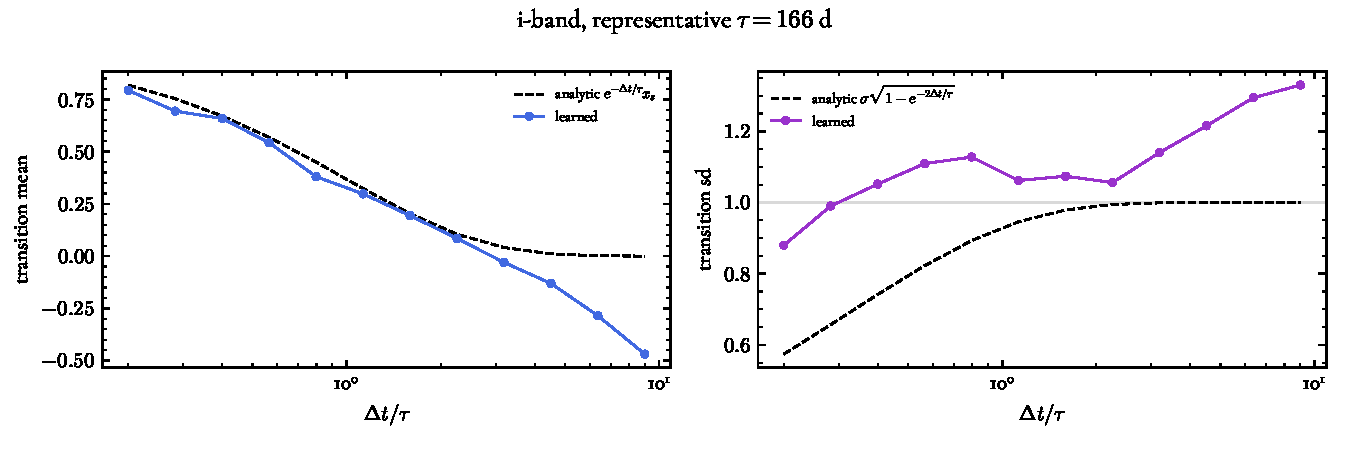
\includegraphics[width=0.9\textwidth]{assets/5_figures/ZTF/ZTF_LearnedTransi.pdf}
        \caption{$i$ band}
        \label{fig:trans_ztf_i}
    \end{subfigure}

    \begin{subfigure}{\textwidth}
        \centering
        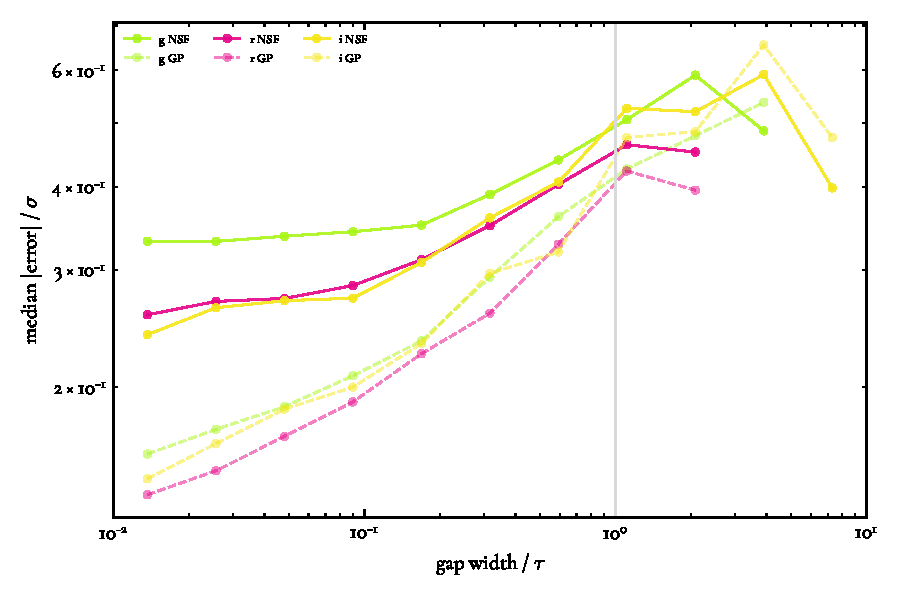
\includegraphics[width=0.5\textwidth]{assets/5_figures/ZTF/ZTF_Error.pdf}
        \caption{Reconstruction error against gap width}
        \label{fig:error_ztf}
    \end{subfigure}

    \caption[The learned transition and reconstruction error under ZTF noise]{\label{fig:trans_ztf} Behaviour of the reconstruction in the ZTF regime. Panels (a)--(c): the learned transition for models trained in each band, as in Figure \ref{fig:trans_fixed}. The learned mean overshoots past zero and the learned standard deviation inflates and does not saturate at unity. Panel (d): the reconstruction error as a function of gap width in units of the damping timescale, for the three bands, compared with the Gaussian process.}
\end{figure}



\section{Application to Real ZTF Light Curves}
\label{sec:realztf}

The method is finally applied to the real ZTF light curves. Since the true signal is unavailable, the reconstruction is tested by masking. A fraction of the observations in each curve is withheld in two forms. Randomly removed isolated points, bracketed by nearby retained observations, test the reconstruction where it is well constrained, while points removed inside contiguous intervals test it across genuine gaps. Before masking, isolated outliers are removed with a local median filter, so that a single discrepant epoch is not mistaken for a real excursion.

The withheld observations play no part in the reconstruction. The retained points alone are used to fit the normalization and, for the Gaussian process, the damping timescale and amplitude. This is the essential difference from the simulated experiments, where the Gaussian process was given the true parameters and acted as an oracle. On real data those parameters are unknown, so the Gaussian process must estimate the timescale and amplitude it conditions on, and it is no longer optimal. Each masked curve is reconstructed by the flow, by this fitted Gaussian process, and by a linear interpolation between observations, which provides a point prediction with no associated uncertainty. The three are compared with the withheld observations.

Because the withheld observations are themselves noisy, a reconstruction of the latent signal should scatter around them rather than pass through them exactly. Each withheld point's measurement variance is therefore added to the predictive interval in quadrature\footnote{The observation is a noisy realization of the latent signal the interval describes, so its variance adds to the predictive variance.} before scoring, equally for the flow and the Gaussian process. Since these points are withheld, their noise enters neither reconstruction, so the adjustment is external to both models.

The results are shown in Table \ref{tab:realztf}, separately for the isolated points and for those inside gaps. On the isolated points both methods are close to calibrated, with coverage between $0.68$ and $0.74$, and the fitted Gaussian process remains close to calibrated on the harder in-gap points as well, at $0.69$ to $0.75$. The reconstruction instead over-covers on the in-gap points, reaching $0.85$ to $0.88$ against the nominal $0.68$, so that across real gaps its intervals are wider than necessary. In accuracy both methods predict the withheld observations to within about one variability amplitude, the Gaussian process being consistently the more accurate; both improve on linear interpolation, and both additionally provide an uncertainty, which interpolation does not. Example reconstructions in the three bands are shown in Figure \ref{fig:ztf_filled}.

\begin{table}[H]
\centering
\caption[Held-out prediction on real ZTF light curves]{\label{tab:realztf} Coverage at the $68\%$ level and RMSE for held-out prediction on real ZTF light curves, scored against the withheld noisy observations, shown separately for randomly removed isolated points and for points removed inside contiguous gaps. The Gaussian process uses parameters fitted to the retained points, and the intervals of both probabilistic methods include the uncertainty of each withheld observation. RMSE is in units of the fitted variability amplitude.}
\begin{tabular}{llcccc}
\hline
\noalign{\smallskip}
& & \multicolumn{2}{c}{Coverage @ $68\%$} & \multicolumn{2}{c}{RMSE} \\
\noalign{\smallskip}
Band & Points & NSF & GP & NSF & GP \\
\noalign{\smallskip}
\hline
\noalign{\smallskip}
\multirow{2}{*}{$g$} & isolated & $0.74$ & $0.73$ & $0.907$ & $0.784$ \\
                     & in-gap   & $0.88$ & $0.74$ & $1.019$ & $0.963$ \\
\noalign{\smallskip}
\multirow{2}{*}{$r$} & isolated & $0.68$ & $0.71$ & $0.995$ & $0.887$ \\
                     & in-gap   & $0.85$ & $0.75$ & $1.080$ & $1.012$ \\
\noalign{\smallskip}
\multirow{2}{*}{$i$} & isolated & $0.73$ & $0.70$ & $0.987$ & $0.940$ \\
                     & in-gap   & $0.85$ & $0.69$ & $1.101$ & $0.999$ \\
\noalign{\smallskip}
\hline
\end{tabular}
\end{table}

\begin{figure}[H]
    \centering
    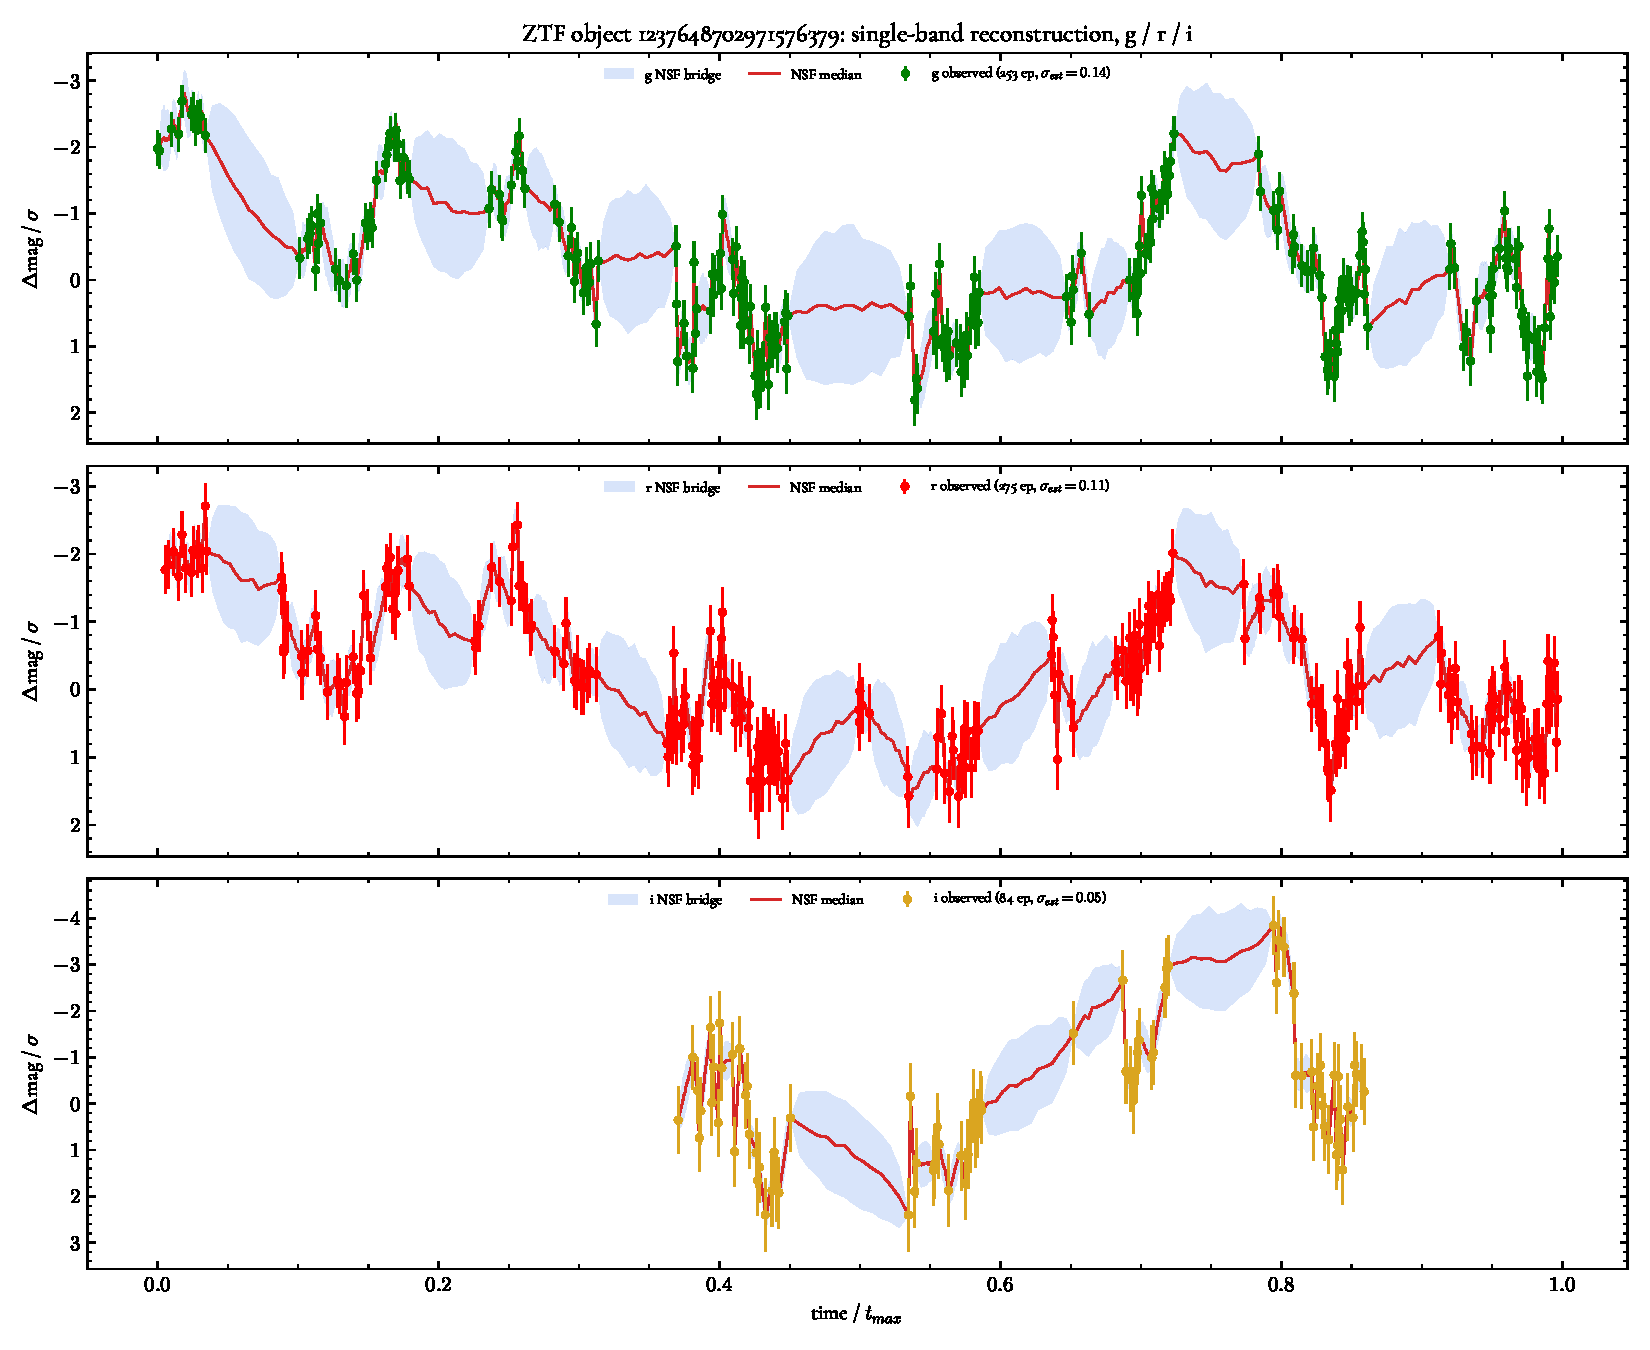
\includegraphics[width=\textwidth]{assets/5_figures/ZTF/ZTF_filled.pdf}
    \caption[Reconstruction of a real ZTF light curve]{\label{fig:ztf_filled} Reconstruction of a real ZTF light curve, showing the observations in green, red and yellow for the  $g$, $r$, and $i$ bands, respectively. The posterior median is shown in red, and the central $68\%$ interval (shaded). The interval widens across the wider gaps in the real cadence.}
\end{figure}


The result on real data appears at first to contradict the simulated evaluation, where the reconstruction was overconfident but, in the simulated experiment, the intervals are compared with the noise-free underlying signal, while here they are compared with noisy observations and are broadened by the observational uncertainty, so the two evaluations measure the coverage of different quantities. What holds across both is that the fitted Gaussian process is a strong and well-calibrated baseline on real data, and that the calibration of the reconstruction depends on how measurement noise is treated.


\section{Discussion}
\label{sec:discussion}

Taken together, the experiments express the limitation of the method. On low noise data, at both fixed and varying timescale, the reconstruction approaches the analytic transition and performs within a few per cent of the Bayes-optimal Gaussian process, so the model and its training objective are solid across a distribution of dynamics. The difficulty appears only when the data carry a significant noise: the reconstruction error tracks the Gaussian process and grows smoothly with gap width, while the coverage departs from nominal. The dependence of this collapse on the number of epochs, deepening a little as more noisy observations are added, together with the loss of the learned transition under noise, points to the model treating the observed magnitudes as if they were the true signal.

%The discussed, natural next step is model that consumes the per-epoch uncertainties, treating each observation as a noisy measurement of a latent state rather than as the state itself and propagate that uncertainty into its predictions. Such a latent formulation, in which the flow describes the evolution of an unobserved signal with a term that relates it to the noisy observations, is the principal direction left for future work. A second direction, motivated by the widest gaps found in the $i$ band, is the extension to multiple bands, since the coordinated variability across bands discussed in Chapter \ref{chap:variability} would allow a gap in one band to be constrained by the others.